\section{Triplet Selection}
As discussed earlier, deep metric learning for joins is a difficult problem for neural networks to learn because it requires that the discrimination of each anchor from all the other hard negatives.  We describe a popular approach batch based approach from the face recognition literature first to contrast it with our mechanism for triplet selection.

\subsection{Batch Based Triple Selection}

\begin{figure}
\subfloat[Batch based\label{batch_selection}]{%
  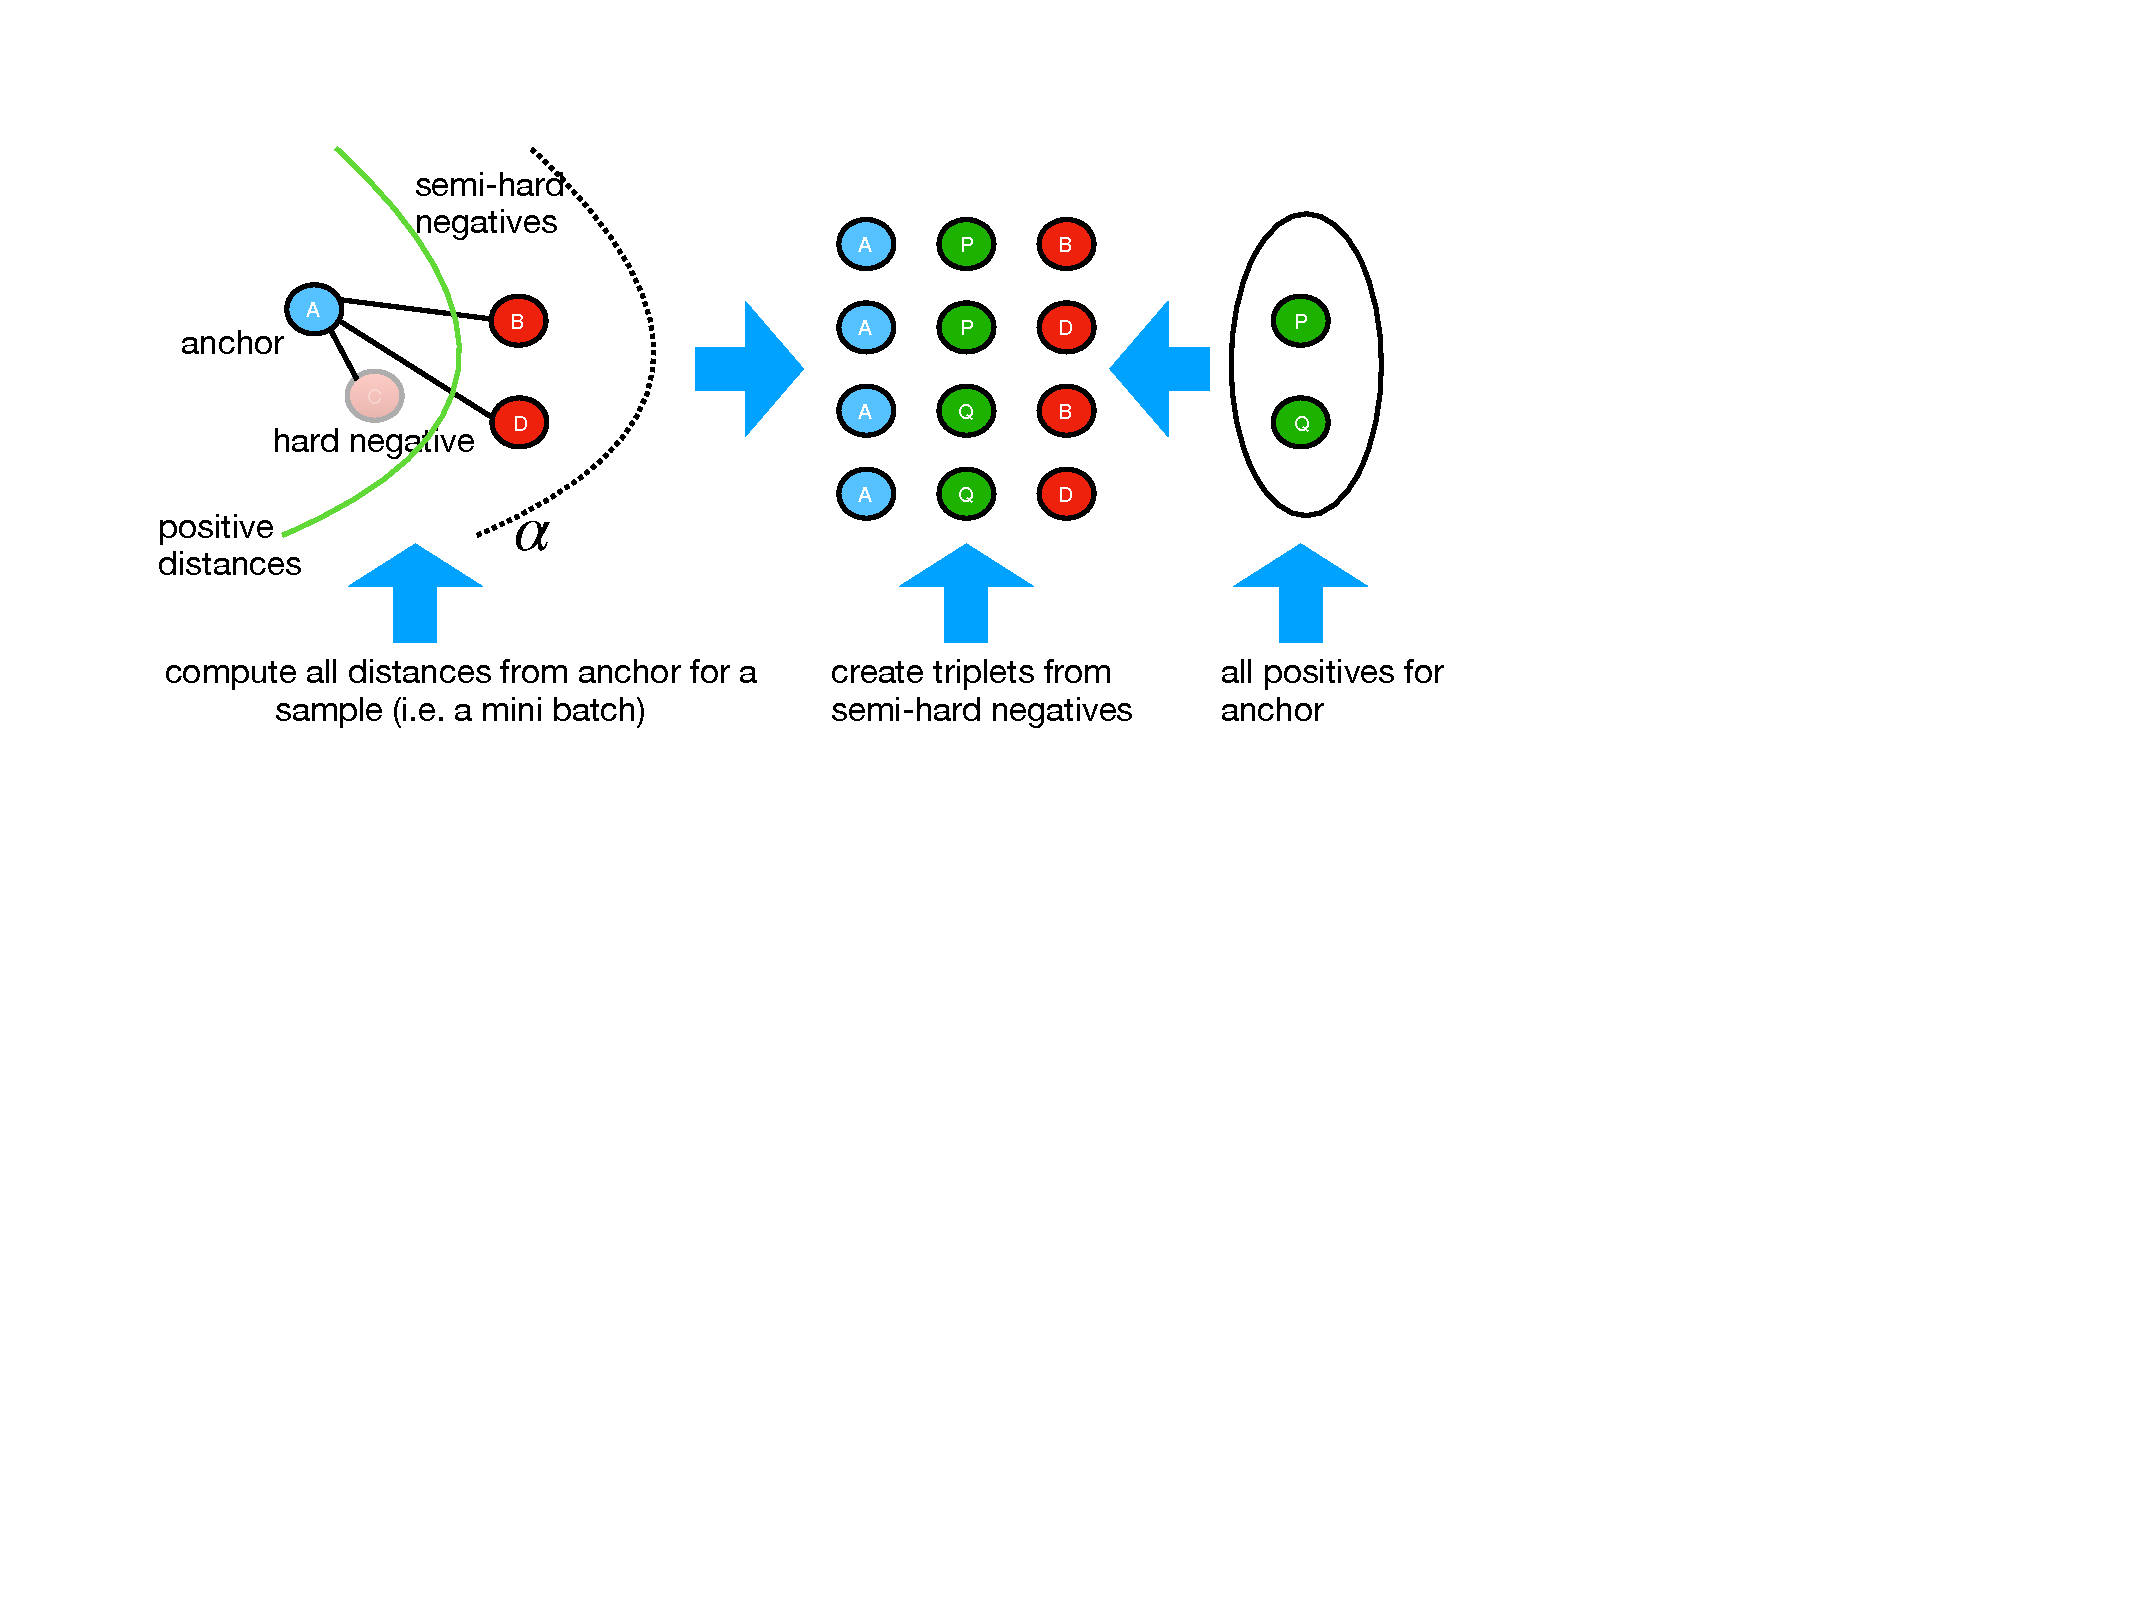
\includegraphics[width=0.5\linewidth]{triplet_selection}
}
~
\subfloat[ANN based\label{ANN_selection}]{%
  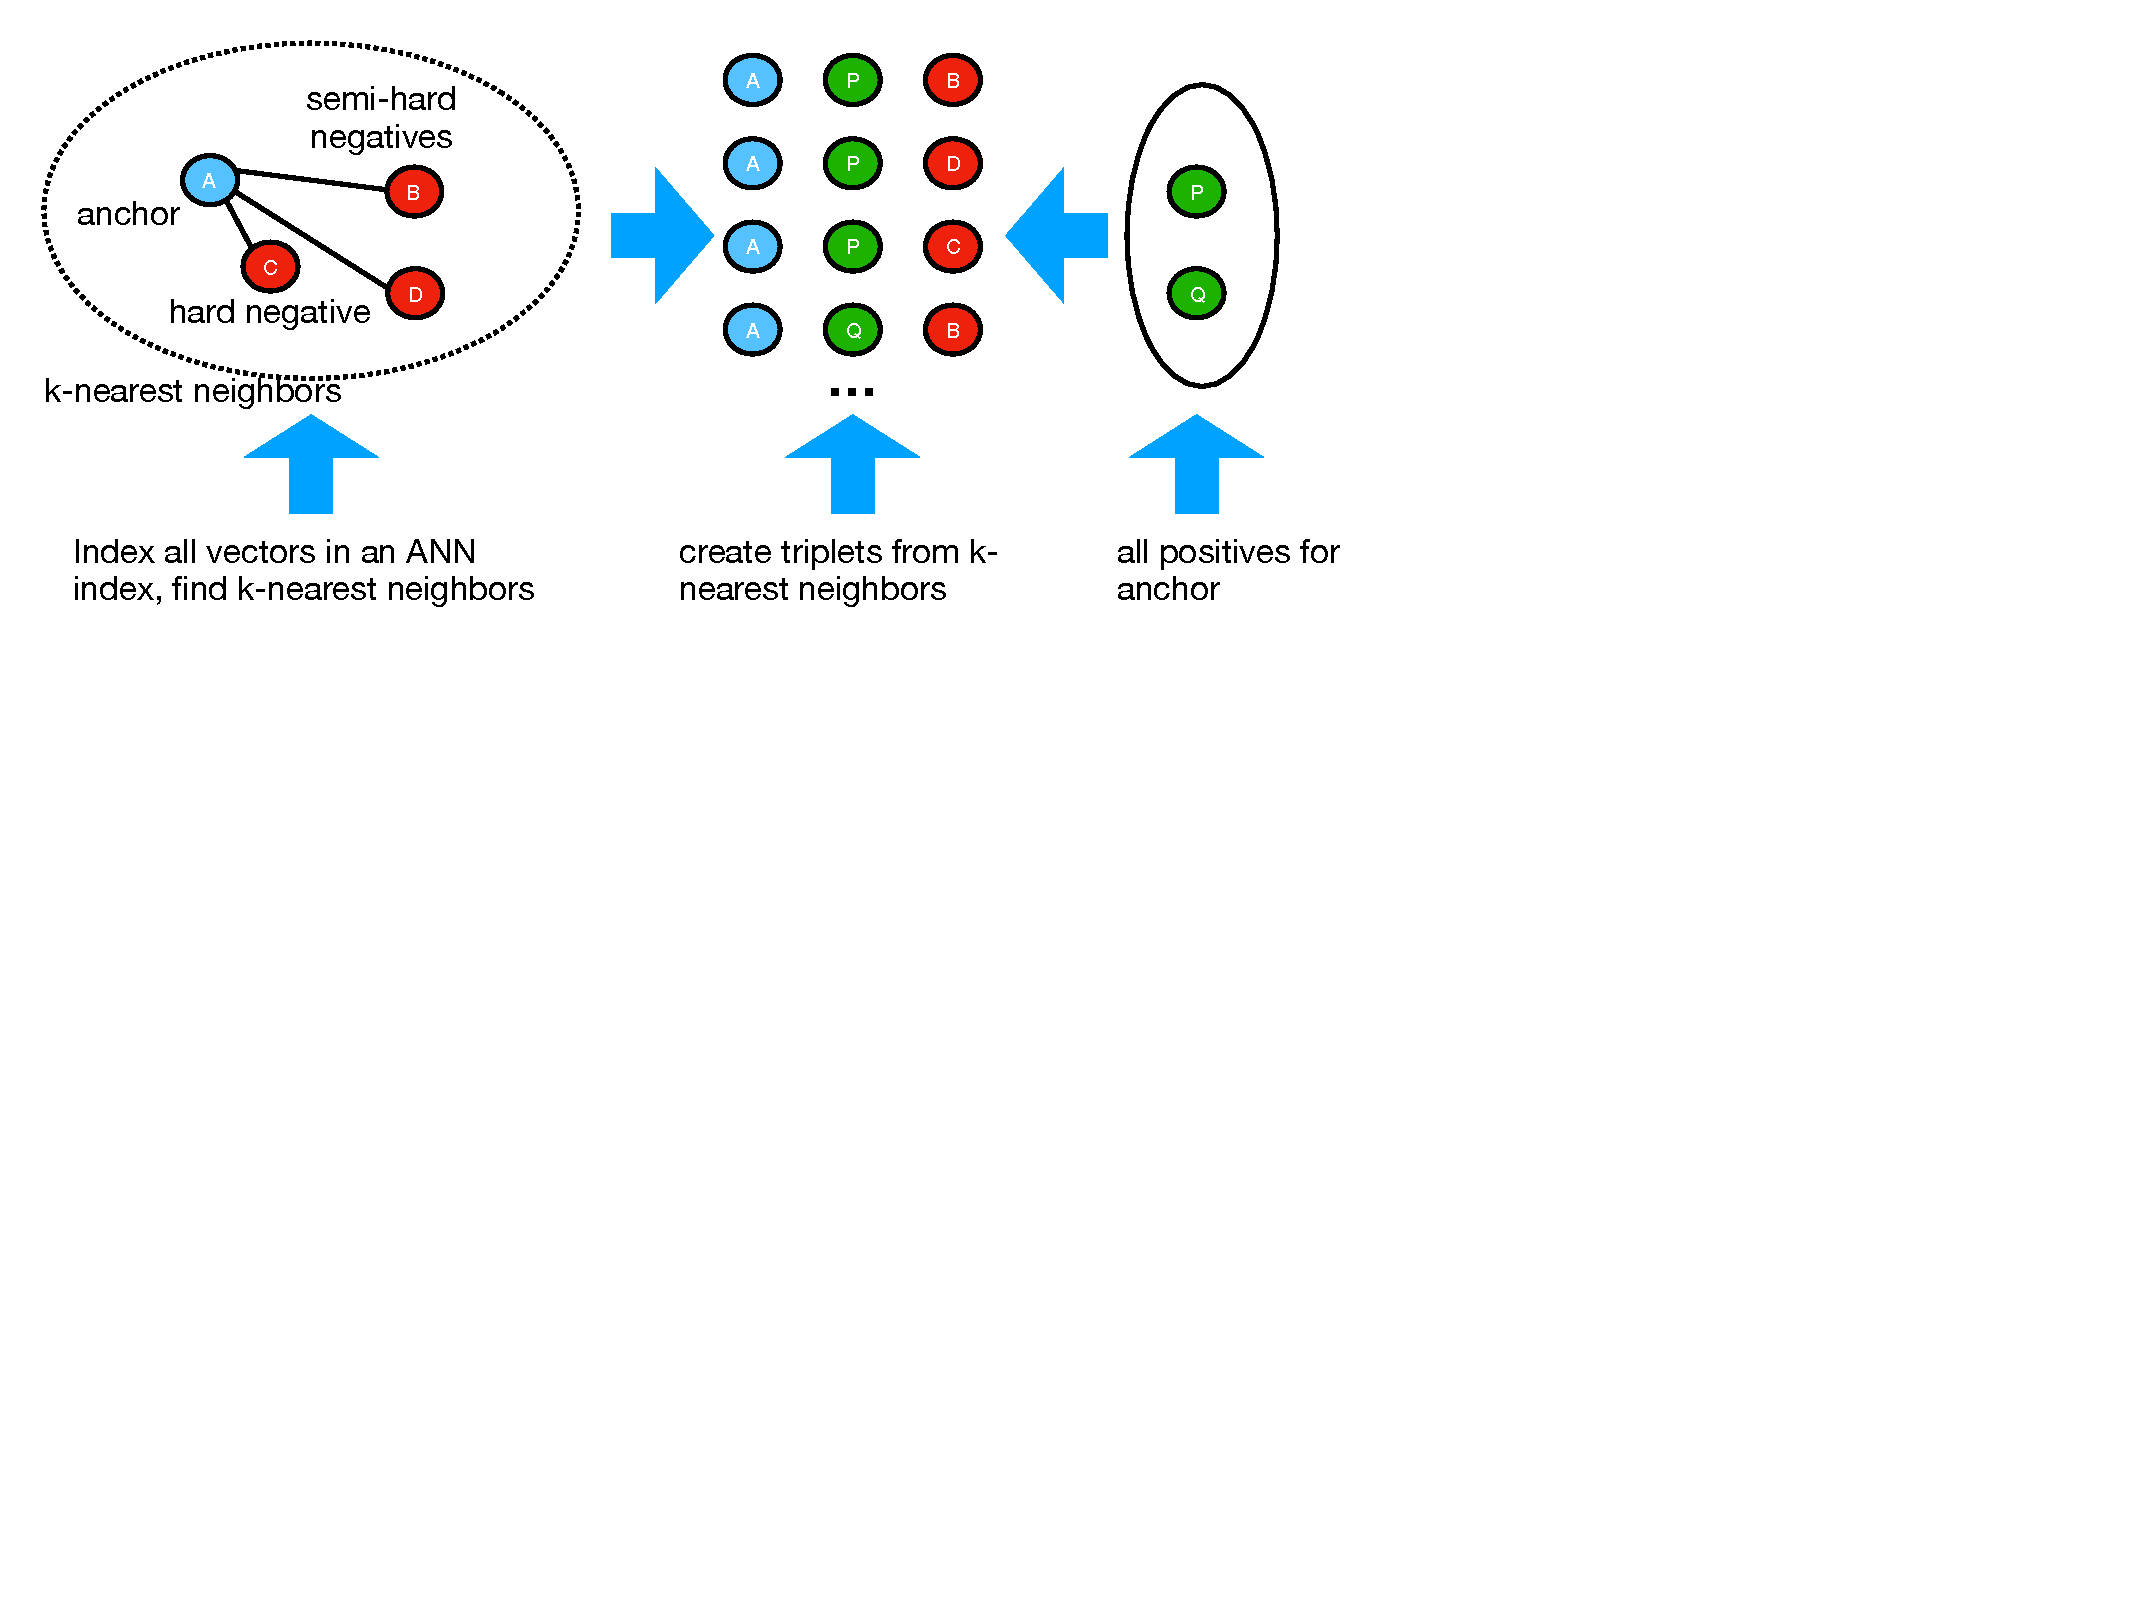
\includegraphics[width=0.5\linewidth]{ANN_selection}
}
\caption{triplet selection}
\label{triplet_selection}
\end{figure}

In Schroff et al.'s work~\cite{DBLP:conf/cvpr/SchroffKP15} they described a mini-batch based triplet selection mechanism for training that has dominated the literature.  Conceptually, sampling the right triplets for fast network learning requires sampling a set of \textit{hard positives} and a set of \textit{hard negatives}, where a hard positive is defined as $argmax^i \| x_{a} - x_{p}^i \|^2$, where $i$ ranges over all $x_p$ and a hard negative is defined as $argmin^i \| x_{a} - x{_n}^i \|^2$, where $i$ ranges over all $x_n$. 

However, it is infeasible to compute these values for the entire dataset.  Calculating hard positives is easy because the number of \textit{positives} is small normally.  Calculating hard negatives is not possible for all but small datasets.  As a result, the triplets can be generated by a mechanism illustrated in Figure~\ref{triplet_selection}.  Instead of focusing on finding \textit{hard positives}, they instead pair every possible positive in the sample shown in the right panel in the figure with selected negatives, since the set of positives is usually quite small.  Furthermore, for negative examples, they try to select \textit{semi-hard negatives} instead of \textit{hard negatives}, where a \textit{semi-hard negative} has the property that $\|x_a - x_p \|^2 < \|x_a - x_n \|^2$ but by a margin smaller than $\alpha$, as shown in figure ~\ref{triplet_selection}.  

%As shown in the figure~\ref{triplet_selection} a \textit{semi-hard negative} is further from the \textit{anchor} than the \textit{positive}, but is not distant enough.  That is, the loss function still needs to move it closer to the margin $\alpha$ that is used in the triplet-loss function.  Schroff et al. further argue selecting \textit{hard negatives} such as $C$ in the figure may in fact lead to bad local minima early on in training, and lead to a collapsed model where the function always learns to return a value of 0, regardless of the pair being considered.

\subsection{Metric Based Triplet Selection}
For the problem of joins, we ideally want the anchor and all of its positives to be clustered closest together and separated from the nearest negatives as clearly as possible.  Approximate nearest neighbor (ANN) indexes are highly efficient methods for selecting the top-K neighbors of a given vector by Euclidean distance, cosine similarity or other distance metrics.  They are based on space partitioning algorithms, such as \textit{k-d trees}, where the vector space is iteratively bisected into two disjoint regions.  The average complexity to query the vectors of a neighbor is $O(log N)$ where N is the number of vectors in the dataset.  Implementations exist now for fast, memory-efficient ANN indexes that scale up to a billion vectors \cite{JDH17} using techniques to compress vectors in memory efficiently.  In our work, we used the Annoy ANN implementation\footnote{\url{https://github.com/spotify/annoy}} in our work which is based on the refinements to \textit{k-d trees} ideas described in \cite{ann_paper}.

Assuming one has the entire dataset indexed in an ANN index, the problem of triplet selection can be simplified by asking the ANN index for the top k-nearest neighbors of an \textit{anchor}, where k is given by the number of triplets that one desires to generate for each anchor.  As in earlier work, selection of \textit{hard positives} is not relevant because all positive data should be used to teach the network the right function.  Selection of negatives is the set of all nearest neighbors that are \textit{negatives}.  There is no explicit attempt to filter out \textit{hard negatives} in the approach.  The overall idea is that the set of negatives that appear in the nearest neighbor set at input are in fact the most important elements for the network to learn to discriminate from positives for a join.  Focusing on these elements, regardless of whether they are \textit{hard} or \textit{semi-hard} should lead to better discrimination for joins.  An ANN-based strategy also provides an important baseline to assess what if any learning was performed by the neural network in mapping input vectors to a different space.
